\documentclass[letterpaper]{article}
\usepackage{natbib}
\usepackage[utf8]{inputenc}
\usepackage{graphicx}
\usepackage{color}
\usepackage{multirow}
\usepackage{amsmath}
\usepackage{array}




\title{Learning Dynamics: Assignement 1}
\author{\Large Hakim Boulahya \\
hboulahy@ulb.ac.be\\
\\
Université Libre de Bruxelles
}

\begin{document}
\maketitle
% \begin{abstract}

% \end{abstract}

\section{Hawk-Dove game}


\begin{figure}[!ht]

\newcolumntype{C}{ >{\centering\arraybackslash} m{4cm} }

\begin{center}
\begin{tabular}{|c|C|C|}
    \hline
     & Hawk & Dove \\[10pt]
    \hline
    Hawk & $\frac{1}{2}(V - D), \quad \frac{1}{2}(V - D)$ & $V, \quad 0$\\[10pt]
    \hline
    Dove & $0, \quad V$ & $\frac{V}{2} - T, \quad \frac{V}{2} - T$\\[10pt]
    \hline
\end{tabular}
\end{center}

\caption{Hawk-Dove game}
\label{fig:hawkdove}
\end{figure}

\subsection{Expected payoff for player 1}

Given player 2’s mixed strategy $\alpha_2$, player 1 expected payoff
for the pure strategy $Hawk(p)$ is:

\begin{equation}
    E_1(H, \alpha_2) = q (\frac{1}{2}(V - D)) + (1 - q)V
    = V - \frac{q}{2}(V - D)
\end{equation}

Given player 2’s mixed strategy $\alpha_2$, player 1 expected payoff
for the pure strategy $Dove(1 - p)$ is:

\begin{equation}
    E_1(D, \alpha_2) = q \cdot 0 + (1 - q)(\frac{V}{2} - T)
    = (1 - q)(\frac{V}{2} - T)
\end{equation}

\subsection{Expected payoff for player 2}

Given player 1’s mixed strategy $\alpha_1$, player 2 expected payoff
for the pure strategy $Hawk(q)$ is:

\begin{equation}
    E_2(H, \alpha_1) = p (\frac{1}{2}(V - D)) + (1 - p)V
    = V - \frac{p}{2}(V - D)
\end{equation}

Given player 1’s mixed strategy $\alpha_1$, player 2 expected payoff
for the pure strategy $Dove(1 - q)$ is:

\begin{equation}
    E_2(D, \alpha_1) = p \cdot 0 + (1 - p)(\frac{V}{2} - T)
    = (1 - p)(\frac{V}{2} - T)
\end{equation}

\subsection{Player 1's mixed strategies}

Since this is a game with two-players two actions
\textit{The linearity implies 3 possible outcomes}:

player 1’s unique best response is the pure strategy $Hawk(p)$ when:

    \begin{alignat*}{2}
    &\iff & E_1(H, \alpha_2) &> E_1(D, \alpha_2) \\
    &\iff &    V - \frac{q}{2}(V - D) &> (1 - q)(\frac{V}{2} - T) \\
    &\iff & V - \frac{V}{2}q + \frac{D}{2}q
    &> \frac{V}{2} - T - \frac{V}{2}q + T \\
    &\iff & q &> -\frac{V}{D}
    \end{alignat*}

player 1’s unique best response is the pure strategy $Dove(1 - p)$ when:

        \begin{alignat*}{2}
        &\iff & E_1(H, \alpha_2) &< E_1(D, \alpha_2) \\
        &\iff & q &< -\frac{V}{D}
        \end{alignat*}

all player 1’s mixed strategies are all best responses when:
        \begin{alignat*}{2}
        &\iff & E_1(H, \alpha_2) &= E_1(D, \alpha_2) \\
        &\iff & q &= -\frac{V}{D}
        \end{alignat*}


\subsection{Player 2's mixed strategies}
\paragraph{}

This game is symmetric, the payoff matrix of player 1 and 2 are the same
($A = B^T$). The strategies of player 2 are the same than the player 1, except
that it depends on $p$ and not on $q$.
\paragraph{}

Player 2's unique best response is pure strategy $Hawk(q)$
when $q > -\frac{V}{D}$,  is pure strategy $Dove(1 - q)$ when
$q < -\frac{V}{D}$ and all mixed strategies are all best response when
$q = -\frac{V}{D}$.

\subsection{Discussions}


\section{Social Dilemma}


\paragraph{}

Figure \ref{fig:brA} represents the expected payoff of $A$ based on her
belief. For example the first column indicates the payoff of $A$ when she
believes that $B$ will defect in all games type.

Since $A$ is sure that each game is equally likely, there is a probability of
$1/3$ that she is in Prisonner's dilemma,
probability of $1/3$ in Stag-Hunt game and probability of $1/3$ in Snowdrift
game.

Figure \ref{fig:brB} represents the best response of player $B$ in all three
games, she doesn't need to form any beliefs since she knows in which game
she is playing.

\begin{figure}[!ht]

\begin{center}
\begin{tabular}{|c|c|c|c|c|c|c|c|c|c|}
    \hline
    & DDD & CCC & CCD & CDC & CDD & DCC & DCD & DDC \\
    \hline
    C & 1/3 & 3 & \textbf{8/3} & 4/3 & 1 & 7/3 & \textbf{\color{red}2} & 2/3 \\
    \hline
    D & \textbf{2/3} & \textbf{4} & 7/3 & \textbf{11/3}
    & \textbf{2} & \textbf{8/3} & 1 & \textbf{\color{red}7/3} \\
    \hline
\end{tabular}
\end{center}

\caption{Expected payoff of player $A$ for all possible combinations of
player $B$’s types}
\label{fig:brA}
\end{figure}

\begin{figure}[!ht]

\begin{center}
\begin{tabular}{|c|c|c||c|c||c|c|}
    \hline
    & C & D & C & D & C & D \\
    \hline
    C & 2 & \textbf{5} & \textbf{5}
    & 2 & 2 & \textbf{5} \\
    \hline
    D & 0 & \textbf{1} & 0 & \textbf{1}
    & \textbf{1} & 0 \\
    \hline
\end{tabular}
\end{center}

\caption{Best response of player $B$ against player $A$ in all games
 (in the following order): Prisonners, Stag-hunt, Snowdrift}
\label{fig:brB}
\end{figure}


\subsection{Payoff function}

\paragraph{}

Let's associate Prisonner's dilemma, Stag-hunt game and Snowdrift game with
the indexes $I = \{1, 2, 3\}$, respectively. The actions
cooperate and defect be the set $A = \{C, D\}$. Let $b_i \; \forall i \in I$,
the beliefs of $A$, with $b_i \in A$ an action.
Let $o_i(x, y) \; \forall i \in I \wedge
\forall x,y \in A$ the outcomes of $A$ for game $i$ and action $x$ for
player $A$ and action $y$ for $B$. The
payoff function is $p(a, b_1, b_2, b_3) \; \forall a \in A$:

\begin{equation}
 p(a, b_1, b_2, b_3) = \frac{1}{3}(o_1(a, b_1)+o_2(a, b_2)+o_3(a, b_3))
\end{equation}

For example the payoff for $A$ action cooperate (C) and beliefs
$b_1 = D, b_2 = D, b_3 = D$, the fist row and column of Figure \ref{fig:brA},
is:

\begin{equation}
    p(C, D, D, D) = \frac{1}{3}(0 + 0 + 1) = 1/3
\end{equation}

Other examples:

\begin{equation}
    p(C, C, C, D) = \frac{1}{3}(2 + 5 + 1) = 8/3
\end{equation}
\begin{equation}
    p(D, C, C, C) = \frac{1}{3}(5 + 2 + 5) = 4
\end{equation}

\subsection{Best response and equilibrium}

\paragraph{}

The best response given the action of all game type for player $A$ are
the bolded values in
Figure \ref{fig:brA}. The best response for all games for player $B$ are
the bolded values in
Figure \ref{fig:brB}. To find the pure Nash Equilibria, we need to match
the best response of $A$ with the best response of $B$ for each beliefs. There
are two pure Nash Equilibria, shows in red in Figure \ref{fig:brA},
$\{C, (DCD)\}$ and $\{D, (DDC)\}$. Indeed, for $\{C, (DCD)\}$,
when $A$ plays action $C$, the best
response of $B$ in Prisonner's dilemma is $D$, in Stag-hunt game it is $C$ and
in Snowdrift game it is $D$, so it is a pure Nash Equilibria. The same
goes for $\{D, (DDC)\}$.

\section{Sequential truel}

\paragraph{}

The diagram representing the subgames are drawn as trees in
Figure \ref{fig:t1}, \ref{fig:t2} and \ref{fig:t3}. When we will refer to $T_1$,
$T_2$ and $T_3$ it means that we are refering to, respectively,
Figure \ref{fig:t1}, \ref{fig:t2} and \ref{fig:t3}. In the subgames,
the action $t(i)$ where $i \in \{A, B, C\}$, means that the current player
is targeting player $i$. The current player can of course not targeting himself.

\paragraph{}

The main game is represented by
$T_1$. As mentioned in the
assignement specifications, the subgames when $A$ fails to hits in intended
target are the same,  it is $T_2$. When in subgame $T_2$, we also found
that when $B$ misses is intended target, the subgames are the same, it is $T_3$.

\begin{figure}[!ht]
 \centerline{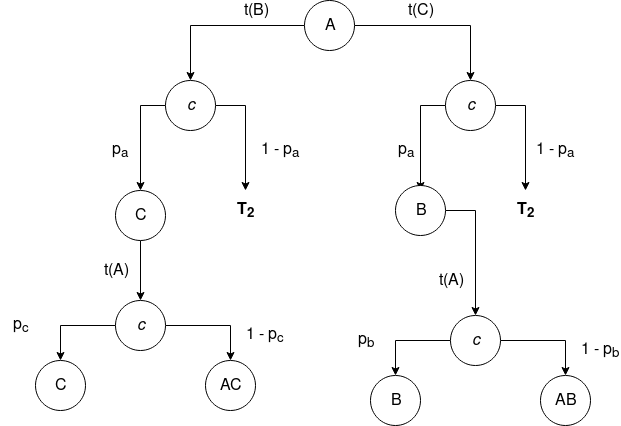
\includegraphics[scale=0.5]{images/T1}}
 \caption{$T_1$, main subgame}
 \label{fig:t1}
\end{figure}

\begin{figure}[!ht]
 \centerline{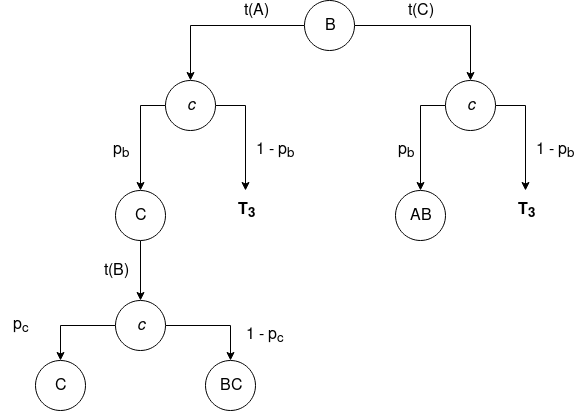
\includegraphics[scale=0.5]{images/T2}}
 \caption{$T_2$, subgame when $A$ misses her intended target}
 \label{fig:t2}
\end{figure}

\begin{figure}[!ht]
 \centerline{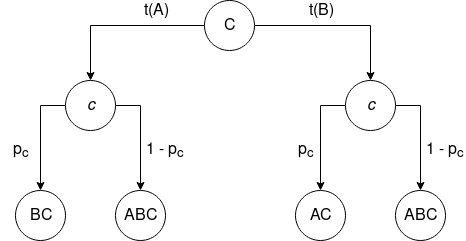
\includegraphics[scale=0.5]{images/T3}}
 \caption{$T_3$, subgame when $A$ and $B$ miss their intended targets}
 \label{fig:t3}
\end{figure}

\subsection{Preferences}
\begin{itemize}
    \item Players prefer outcomes with fewer people
    \item Players prefer to stay alive
\end{itemize}


\subsection{Subgame perfect equilibria}

\paragraph{C equilibrium in $T_3$}

To find the SPE, we have to use the backward induction, so we need to find
the SPE of $T_3$ first. Player $C$ always stay alive whatever target she is
choosing. The SPE is $t(A)$ if $p_a > p_b$, and $t(B)$ if $p_b > p_a$.

\paragraph{B equilibrium in $T_2$}

Let's consider subgame $T_2$. Player $B$ needs either to target $A$
or target $C$. If $B$ targets $A$, she has less chance to survive because,
since next turn $C$ will play and will still be alive whatever the result is
of this shoot, so it $B$ will always target $C$ in $T_3$.
Formally, if $B$ misses her outcome will be the same, because it will have
the SPE of subgame $T_3$, which is unique.
If $B$ targets $A$ and hits her, she has
a probabilty of $1 - p_c$ to stay alive. If $B$ targets $C$ and hits her, she
has a probablity of $1$ to stay alive. So $B$ will always choose to target $C$.

\paragraph{A equilibrium in $T_1$}

Let's consider the full game, subgame $T_1$. Intuitively, it is best for
$A$ to target the player with the biggest probability, because she will have
more chance to stay alive if she manage to eliminate the strongest opponent.
Formally, if $A$ misses her intended target, the outcome will be the same
since $T_2$ has an unique SPE. If $A$ targets $B$ and hits her, she has
a probability of $1 - p_c$ to stay alive, because $C$ is
the remaining shooter and has a probability of $1 - p_c$ to fail.
If $A$ targets $C$ and hits her,
she has a probability of $1 - p_b$ to stay alive, because $B$ is
the remaining shooter and has a probability of $1 - p_b$ to fail.
So $A$ targets $B$ if
$ (1 - p_c) > (1 - p_b)$, which can be simplify as
$p_c < p_b$, and $A$ targets $C$
if $(1 - p_b) > (1 - p_c)$, which can be simplify as $p_b < p_c$.


\paragraph{Weakness is strength}

In the previous paragraph, we explained that if $p_c > p_b$
$A$ will target $C$. If $C$ is the target, the her probablity of survival
is the probability that $A$ misses and $B$ misses,
formally:
\begin{equation}
    \label{weak:1}
    (1 - p_a)(1 - p_b) = 1 - p_b - p_a + p_ap_b = 1 - p_a - p_b(1 - p_a)
\end{equation}
If $p_b > p_c$ $A$ will target $B$, then $C$ chance of survival is $A$ hits
her target and $C$ will be the last player with a bullet or $A$
misses her target and $B$ misses also her target. Formally:

\begin{equation}
    \label{weak:2}
    p_a + (1 - p_a)(1 - p_b) =
    p_a + 1 - p_b - p_a + p_ap_b = 1 - p_b(1 - p_a)
\end{equation}

The difference between the probablity (\ref{weak:1}) and (\ref{weak:2}), is that
(\ref{weak:1}) is decreasing (\ref{weak:2})
with $p_a$, so (\ref{weak:1}) will
always be smaller that (\ref{weak:2}). The probablity of
survival of $C$ when $p_c > p_b$ will always be smaller than
the probability of survival of $C$ when $p_b > p_c$. $C$ is always better off
when $p_b > p_c$.

\end{document}
